\documentclass[../main.tex]{subfiles}

\begin{document}
	\subsection{Centered Inverter}
	{
		\begin{tcolorbox}[colback=gray!5!white,colframe=gray!75!black]
			Plot the static transfer function for a centered inverter. Deduce the noise margin on the input low state and high state.
		\end{tcolorbox}
	
		\begin{lstlisting}
			.include cmosws.mod
			
			Vin 1 0 dc 1V
			Vdd 2 0 dc 3.3V
			M1  3 1 0 0 MODN L=0.6U W=3.0U
			M2  2 1 3 2 MODP L=0.6U W=6.0U
			
			.dc Vin 0 3.3 50mV
			.end
		\end{lstlisting}
		
		\begin{figure}[H]
			\centering
			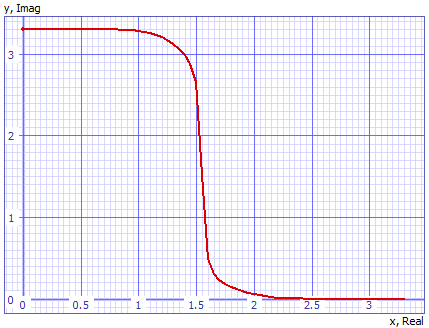
\includegraphics[width=0.5\textwidth]{plots/Q3.png}
			\caption{Transfer function for centered inverter}
		\end{figure}
		
		From the graphic, we have
		\begin{itemize}
			\item $V_{IL} = 0,92$V (maximum $V_{in}$ for which $V_{out}$ is high)
			\item $V_{IH} = 2,3$V (minimum $V_{in}$ for which $V_{out}$ is low)
			\item and we consider $V_{OL} = 0$V and $V_{OH} = 3,3$V.
		\end{itemize}
		
		We conclude that
		\begin{itemize}
			\item $NML = V_{IL} - V_{OL} = 0,92$V
			\item $NMH = V_{OH} - V_{IH} = 3,3 - 2,3 = 1$V
		\end{itemize}
		
		We observe that $W_p = 2W_n$ did not give us a perfectly centered inverter, we expected $NML = NMH$.
	}
\end{document}